% !TeX document-id = {5c05c331-134f-48f1-8db3-fd32c67a647b}
%%%%%%%%%%%%%%%%%%%%%%%%%%%%%%%%%%%%%%%%%
% Journal Article
% LaTeX Template
% Version 2.0 (February 7, 2023)
%
% This template originates from:
% https://www.LaTeXTemplates.com
%
% Author:
% Vel (vel@latextemplates.com)
%
% License:
% CC BY-NC-SA 4.0 (https://creativecommons.org/licenses/by-nc-sa/4.0/)
%
% NOTE: The bibliography needs to be compiled using the biber engine.
%
%%%%%%%%%%%%%%%%%%%%%%%%%%%%%%%%%%%%%%%%%

% Magic comments for TeXStudio
% !TeX program = pdflatex
% !BIB program = biber
% !TeX encoding = utf8
% !TeX spellcheck = en_US

%----------------------------------------------------------------------------------------
%	PACKAGES AND OTHER DOCUMENT CONFIGURATIONS
%----------------------------------------------------------------------------------------

\documentclass[
a4paper, % Paper size, use either a4paper or letterpaper
10pt, % Default font size, can also use 11pt or 12pt, although this is not recommended
unnumberedsections, % Comment to enable section numbering
twoside, % Two side traditional mode where headers and footers change between odd and even pages, comment this option to make them fixed
onecolumn,
]{LTJournalArticle}

\bibliography{sample.bib} % BibLaTeX bibliography file

\runninghead{} % A shortened article title to appear in the running head, leave this command empty for no running head

\footertext{} % Text to appear in the footer, leave this command empty for no footer text

\setcounter{page}{1} % The page number of the first page, set this to a higher number if the article is to be part of an issue or larger work

\usepackage{graphicx} 

% Main header file
% % % % % % % % % % % % % % % % % % % % % % % % % % % % % % % % % % % % % % % % %
%
% OSTReport -- Additional packages frequently used in reports
%
% % % % % % % % % % % % % % % % % % % % % % % % % % % % % % % % % % % % % % % % %

% Mathematical equations
\usepackage{amsmath}
\usepackage{amssymb}
\usepackage{bm}
\usepackage{MnSymbol}
%\usepackage{breqn}

% Tables
\usepackage{multirow}
\usepackage{tabularx}
\usepackage{booktabs}

% Figures
\usepackage{pdfpages}
\usepackage{epstopdf}
%\usepackage[outdir=./]{epstopdf}

% Quotation marks
\usepackage{csquotes}
\setquotestyle[quotes]{german}

% Si Units
\usepackage{siunitx}
\sisetup{detect-all,sticky-per,per-mode=symbol}

% Multicolumn documents and sections
\usepackage{multicol}

\PassOptionsToPackage{svgnames,x11names,dvipsnames}{xcolor}
\usepackage[most]{tcolorbox}

%----------------------------------------------------------------------------------------
%	TITLE SECTION
%----------------------------------------------------------------------------------------

\title{Digital Signal Processing \\ Summary} % Article title, use manual lines breaks (\\) to beautify the layout

% Authors are listed in a comma-separated list with superscript numbers indicating affiliations
% \thanks{} is used for any text that should be placed in a footnote on the first page, such as the corresponding author's email, journal acceptance dates, a copyright/license notice, keywords, etc
\author{%
	Nathan Hoffman\textsuperscript{1}, Antoine Biebyck\textsuperscript{1}, Valentina Jakob\textsuperscript{1}
}

% Affiliations are output in the \date{} command
\date{\footnotesize\textsuperscript{\textbf{1}}University of Bern\\ }

% Full-width abstract
\renewcommand{\maketitlehookd}{%
	\begin{abstract}
		\noindent This is a summary of the lecture "Introduction to Digital Signal Processing" which was held in the HS 2023.
	\end{abstract}
}

\usepackage{makecell}

\renewcommand\theadalign{bc}
\renewcommand\theadfont{\bfseries}
\renewcommand\theadgape{\Gape[4pt]}
\renewcommand\cellgape{\Gape[4pt]}

%----------------------------------------------------------------------------------------

\begin{document}
	
	\maketitle % Output the title section
	
	%----------------------------------------------------------------------------------------
	%	TABLE OF CONTENTS
	%----------------------------------------------------------------------------------------
	{
		%	\markleft{\contentsname}
		\pdfbookmark[0]{\contentsname}{\contentsname}
		\hypersetup{hidelinks}    % Don't format as links
		\tableofcontents
	}
	
	%----------------------------------------------------------------------------------------
	%	ARTICLE CONTENTS
	%----------------------------------------------------------------------------------------
	% !TeX document-id = {5c05c331-134f-48f1-8db3-fd32c67a647b}
%%%%%%%%%%%%%%%%%%%%%%%%%%%%%%%%%%%%%%%%%
% Journal Article
% LaTeX Template
% Version 2.0 (February 7, 2023)
%
% This template originates from:
% https://www.LaTeXTemplates.com
%
% Author:
% Vel (vel@latextemplates.com)
%
% License:
% CC BY-NC-SA 4.0 (https://creativecommons.org/licenses/by-nc-sa/4.0/)
%
% NOTE: The bibliography needs to be compiled using the biber engine.
%
%%%%%%%%%%%%%%%%%%%%%%%%%%%%%%%%%%%%%%%%%

% Magic comments for TeXStudio
% !TeX program = pdflatex
% !BIB program = biber
% !TeX encoding = utf8
% !TeX spellcheck = en_US
%----------------------------------------------------------------------------------------
%	ARTICLE CONTENTS
%----------------------------------------------------------------------------------------
\section{Lecture 1 - Signals and Systems}
\subsection{What is a signal?}
Variations of a physical quantity that can be manipulated, stored, or transmitted by physical processes. It is a function of time and space!
\newline Mathematical representation of signals (1D, 2D):
\begin{itemize}
	\item Continuous time signal $x(t), p(x,y)$
	\item Discrete time signal $x[n] = x[nT_s], p[m,n] = p[m\Delta_x ,n\Delta_y] $ with $T_s$ and $\Delta_x$, $\Delta_y$ being the sampling period
\end{itemize}
\subsection{What is a system?}
Something that can manipulate, change, record, or transmit signals. Systems operate on signals to produce new signals or new signal representations.
\newline A sampler is defined as a system whose input is a continuous-time signal x(t) and whose output is the corresponding sequence of samples, defined by the equation x[n] = x(nT) which simply states that the sampler “takes an instantaneous snapshot” of the continuous- time input signal once every T seconds.
\subsection{Sinusoids}
They are the basic building blocks of signals and systems. General formula:
\begin{equation}
	x(t)=A \cos(\omega_0 t+\varphi)=A \cos(2\pi f_0 t+\varphi)
\end{equation}
with $A$ the amplitude, $\omega_0$ the radian frequency, $f_0$ the cyclic frequency, the period $T_0 = \dfrac{2 \pi}{\omega_0} = \dfrac{1}{f_0}$ and $\varphi$ the phase.
\newline A tuning fork is a very simple and familiar system for generating a sinusoidal signal.
\subsection{Review of Sine and Cosine Functions}
\begin{figure}[h]
	\centering
	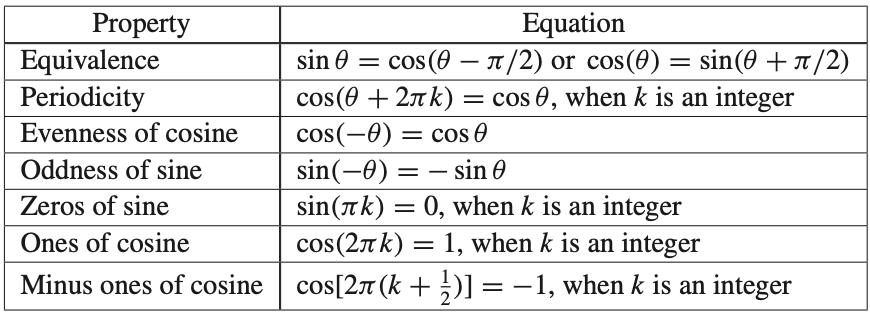
\includegraphics[width=0.7\linewidth]{Figures/DSP_Figures_Lecture1/Basic_Properties_SinCosine}
	\caption{Basic properties of the sine and cosine functions}
	\label{fig:basicpropertiessincosine}
\end{figure}
\begin{figure}[h]
	\centering
	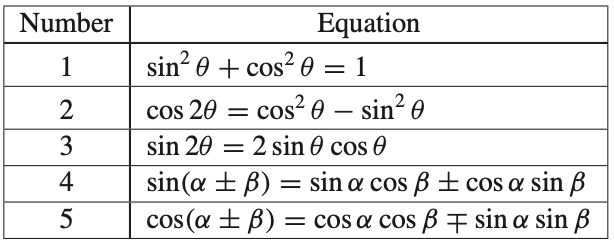
\includegraphics[scale=0.80]{Figures/DSP_Figures_Lecture1/Trigonometric_Identities}
	\caption{Some basic trigonometric identities}
	\label{fig:trigonometric_identities}
\end{figure}
\subsection{Time and Phase Shift}
Time-shifting
\begin{itemize}
	\item Whenever a signal can be expressed in the form $x_1 (t) = s(t - t_1)$, we say that $x_1 (t)$ is a time-shifted version of $s(t)$. If $t_1$ is a positive number, then the shift is to the right, and we say that the signal $s(t)$ has been delayed in time. When $t_1$ is a negative number, then the shift is to the left, and we say that the signal $s(t)$ was advanced in time.
\end{itemize}
Phase shift
\begin{itemize}
	\item The phase parameter $\varphi$ (together with the frequency) determines the time locations of the maxima and minima of a cosine wave, as well as the zero crossings in-between. We can relate the time delay to phase.
	\item Let $x_0 (t) = A \cos(\omega_0 t)$ denote a cosine signal with zero phase. A delay of $x_0 (t)$ can be converted to a phase $\varphi$ by making the following comparison:
	\begin{equation}
		x_0 (t - t_1 ) = A \cos(\omega_0 (t - t_1 )) = A \cos(\omega_0 t + \varphi)
	\end{equation}
	with $\varphi=-\omega_0 t_1$. Notice that the phase is negative when the time shift $t_1$ is positive (a delay)
	\item We can also express the phase in terms of the period $T_0 = \dfrac{1}{f_0}$
	\begin{equation}
		\varphi=-\omega_0 t_1 = -2\pi \dfrac{t_1}{T_0}
	\end{equation}
\end{itemize}





	% !TeX document-id = {5c05c331-134f-48f1-8db3-fd32c67a647b}
%%%%%%%%%%%%%%%%%%%%%%%%%%%%%%%%%%%%%%%%%
% Journal Article
% LaTeX Template
% Version 2.0 (February 7, 2023)
%
% This template originates from:
% https://www.LaTeXTemplates.com
%
% Author:
% Vel (vel@latextemplates.com)
%
% License:
% CC BY-NC-SA 4.0 (https://creativecommons.org/licenses/by-nc-sa/4.0/)
%
% NOTE: The bibliography needs to be compiled using the biber engine.
%
%%%%%%%%%%%%%%%%%%%%%%%%%%%%%%%%%%%%%%%%%

% Magic comments for TeXStudio
% !TeX program = pdflatex
% !BIB program = biber
% !TeX encoding = utf8
% !TeX spellcheck = en_US
%----------------------------------------------------------------------------------------
%	ARTICLE CONTENTS
%----------------------------------------------------------------------------------------
\section{Lecture 2 - Complex Exponentials and Phasors}
	
	
	
	%----------------------------------------------------------------------------------------
	%	 REFERENCES
	%----------------------------------------------------------------------------------------
	
	\printbibliography % Output the bibliography
	
	%----------------------------------------------------------------------------------------
	
\end{document}
